\frame{
    \frametitle{Validity of Linear Combinations at Truth-Level}
    \begin{columns}
        \begin{column}{0.4\textwidth}
            \begin{center} 
            {\tiny Basis Set}

            \resizebox{0.2\textheight}{!}{\begin{tabular}{ |l|l|l| }
                \hline
                \textbf {$\kappa_{2V}$} & \textbf {$\kappa_\lambda$} & \textbf {$\kappa_V$} \\
                \hline
                1.  &  1. &  1.  \\
                1.5 &  1. &  1.  \\
                2.  &  1. &  1.  \\
                1.  &  0. &  1.  \\
                1.  & 10. &  1.  \\
                1.  &  1. &  1.5 \\
                \hline
            \end{tabular}} \end{center}

            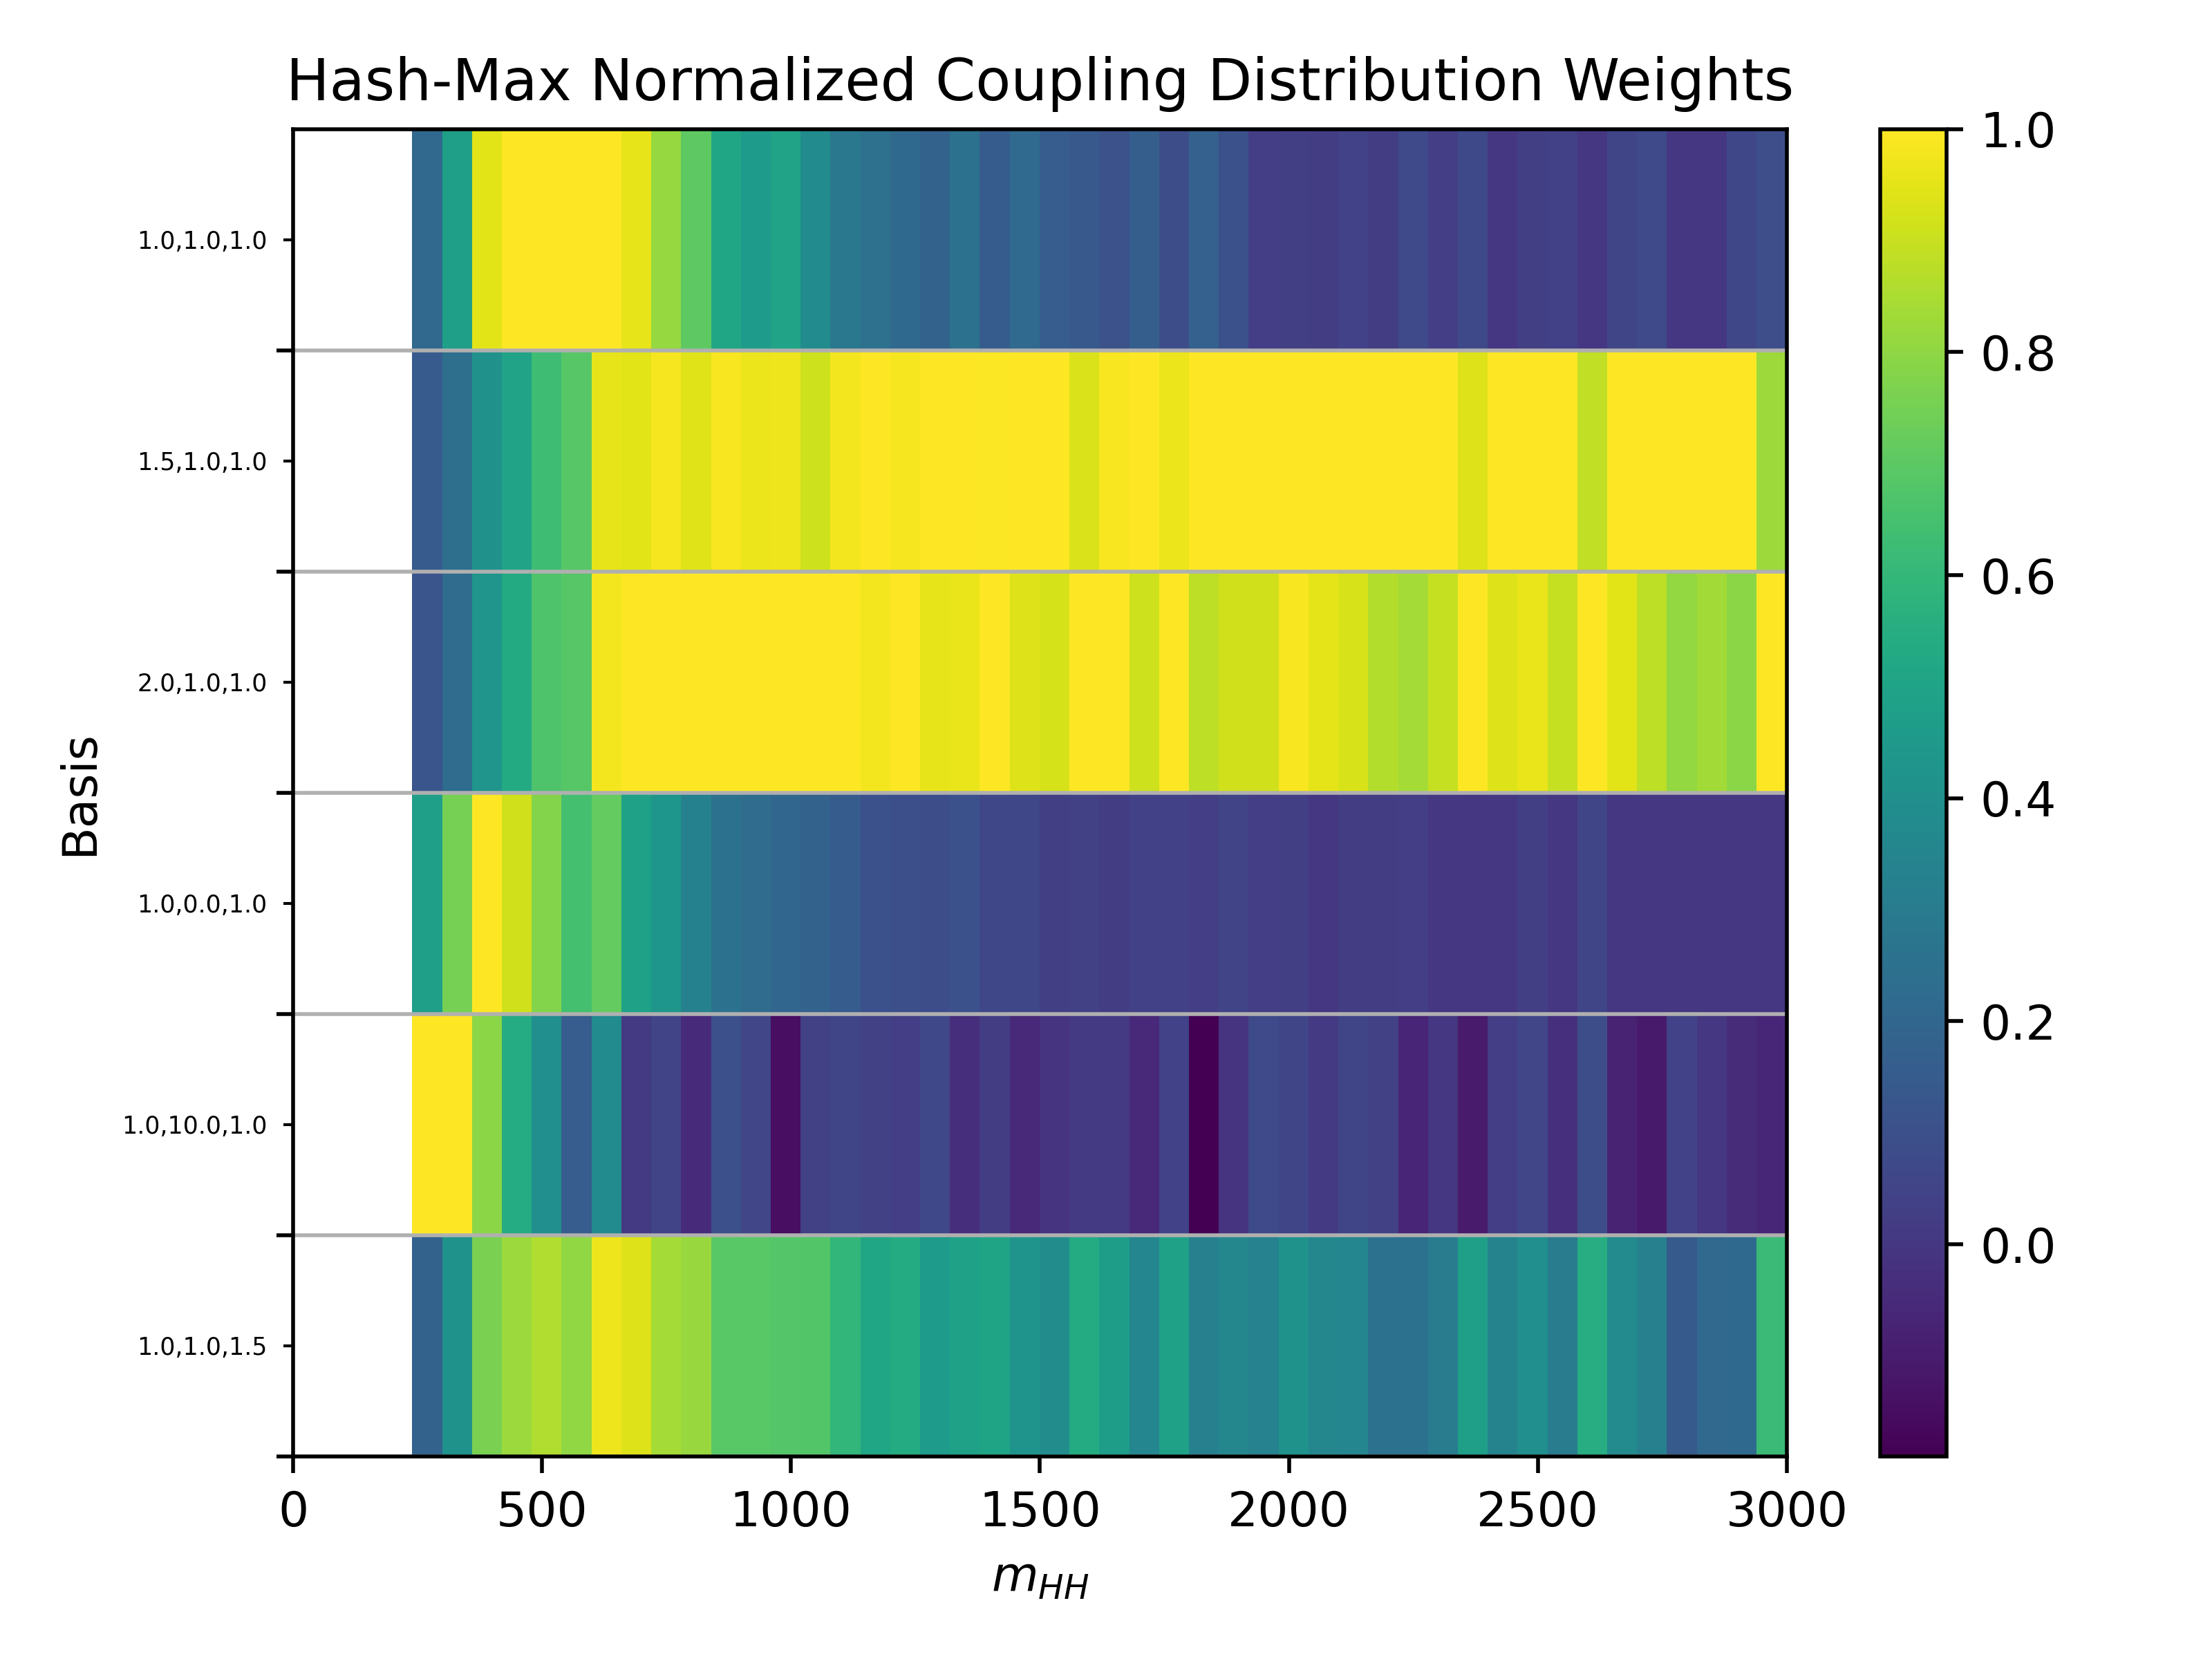
\includegraphics[width=\linewidth,height=\textheight,keepaspectratio]
                {coupling_scan_auto_chosenR1_hash_max}

        \end{column}
        \begin{column}{0.6\textwidth}
            \resizebox{0.8\textwidth}{!}{ \begin{minipage}{1.0\textwidth}
            Linear Combination Equation

            \vspace{10mm}

            {\tiny $
\left|{A{\left(1,1,1 \right)}}\right|^{2} \left(2 \kappa_{2V}^{2} + \frac{136 \kappa_{2V} \kappa_{V}^{2}}{15} - \frac{241 \kappa_{2V} \kappa_{V} \kappa_{\lambda}}{15} - \frac{166 \kappa_{V}^{4}}{15} + \frac{773 \kappa_{V}^{3} \kappa_{\lambda}}{45} - \frac{\kappa_{V}^{2} \kappa_{\lambda}^{2}}{9}\right)
+ \left|{A{\left(1.5,1,1 \right)}}\right|^{2}  \left(- 4 \kappa_{2V}^{2} - \frac{20 \kappa_{2V} \kappa_{V}^{2}}{3} + \frac{56 \kappa_{2V} \kappa_{V} \kappa_{\lambda}}{3} + \frac{32 \kappa_{V}^{4}}{3} - \frac{56 \kappa_{V}^{3} \kappa_{\lambda}}{3}\right)
+ \left|{A{\left(2,1,1 \right)}}\right|^{2} \left(2 \kappa_{2V}^{2} + \frac{4 \kappa_{2V} \kappa_{V}^{2}}{3} - \frac{19 \kappa_{2V} \kappa_{V} \kappa_{\lambda}}{3} - \frac{10 \kappa_{V}^{4}}{3} + \frac{19 \kappa_{V}^{3} \kappa_{\lambda}}{3}\right)
+ \left|{A{\left(1,0,1 \right)}}\right|^{2} \left(\frac{42 \kappa_{2V} \kappa_{V}^{2}}{25} - \frac{42 \kappa_{2V} \kappa_{V} \kappa_{\lambda}}{25} - \frac{17 \kappa_{V}^{4}}{25} + \frac{29 \kappa_{V}^{3} \kappa_{\lambda}}{50} + \frac{\kappa_{V}^{2} \kappa_{\lambda}^{2}}{10}\right)
+ \left|{A{\left(1,10,1 \right)}}\right|^{2} \left(- \frac{\kappa_{2V} \kappa_{V}^{2}}{75} + \frac{\kappa_{2V} \kappa_{V} \kappa_{\lambda}}{75} + \frac{\kappa_{V}^{4}}{75} - \frac{11 \kappa_{V}^{3} \kappa_{\lambda}}{450} + \frac{\kappa_{V}^{2} \kappa_{\lambda}^{2}}{90}\right) 
+ \left|{A{\left(1,1,1.5 \right)}}\right|^{2} \left(- \frac{16 \kappa_{2V} \kappa_{V}^{2}}{15} + \frac{16 \kappa_{2V} \kappa_{V} \kappa_{\lambda}}{15} + \frac{16 \kappa_{V}^{4}}{15} - \frac{16 \kappa_{V}^{3} \kappa_{\lambda}}{15}\right)
$
}
            \end{minipage}}
        \end{column}
    \end{columns}
}

\displaythree{Truth Combination Plots}
{Note that variation (1,1,1) is among the basis states and only present as a sanity check.}
{truth_comb_cvv1p0cl1p0cv1p0}
{truth_comb_cvv1p0cl20p0cv1p0}
{truth_comb_cvv1p0cl1p0cv0p5}
 
\displaythree{More Truth Combination Plots}{}
{truth_comb_cvv0p0cl0p0cv1p0}
{truth_comb_cvv0p0cl1p0cv1p0}
{truth_comb_cvv0p5cl1p0cv1p0}
 
\displaythree{Yet More Truth Combination Plots}{}
{truth_comb_cvv1p0cl2p0cv1p0}
{truth_comb_cvv1p0cl5p0cv1p0}
{truth_comb_cvv3p0cl1p0cv1p0}
